% questions.tex —— 2009 年·普通高等学校招生考试·安徽卷·文科 · 题目内容片段（无答案）
% 由 tools/generate_projects.py 依来源总账自 2009/2009_数学真题_安徽文_试题.md 生成，勿手改（改源 MD 后重跑）


状态：needs-review；依固定候选 PDF 两页（印刷页 497–498）逐题核验，图形已矢量重绘，正式构建与逐页验收见回执。源未标分值，不补分值。原卷第 17 题称「两种小麦各种植了 $25$ 亩」，但印出的亩产数据 A、B 各 $24$ 个，按原页照录并在题注中说明。第 21 题原页印作「$\mathrm e=0.71828\cdots$」，显系 $2.71828$ 的排印脱字，按原页照录并在解析中说明，不影响所问值域。

\gkpart{一、选择题}

\begin{question}
\gkti{1}$\mathrm i$ 是虚数单位，$\mathrm i(1+\mathrm i)$ 等于（　）

（A）$1+\mathrm i$

（B）$-1-\mathrm i$

（C）$1-\mathrm i$

（D）$-1+\mathrm i$

\end{question}
\begin{question}
\gkti{2}若集合 $A=\left\{x\mid (2x+1)(x-3)<0\right\}$，$B=\{x\in\mathbf N_+\mid x\leqslant5\}$，则 $A\cap B$ 是（　）

（A）$\{1,2,3\}$

（B）$\{1,2\}$

（C）$\{4,5\}$

（D）$\{1,2,3,4,5\}$

\end{question}
\begin{question}
\gkti{3}不等式组 $\begin{cases}x\geqslant0,\\ x+3y\geqslant4,\\ 3x+y\leqslant4\end{cases}$ 所表示的平面区域的面积等于（　）

（A）$\frac32$

（B）$\frac23$

（C）$\frac43$

（D）$\frac34$

\end{question}
\begin{question}
\gkti{4}「$a+c>b+d$」是「$a>b$ 且 $c>d$」的（　）

（A）必要不充分条件

（B）充分不必要条件

（C）充分必要条件

（D）既不充分也不必要条件

\end{question}
\begin{question}
\gkti{5}已知 $\{a_n\}$ 为等差数列，$a_1+a_3+a_5=105$，$a_2+a_4+a_6=99$，则 $a_{20}$ 等于（　）

（A）$-1$

（B）$1$

（C）$3$

（D）$7$

\end{question}
\begin{question}
\gkti{6}下列曲线中离心率为 $\dfrac{\sqrt6}{2}$ 的是（　）

（A）$\frac{x^2}{2}-\frac{y^2}{4}=1$

（B）$\frac{x^2}{4}-\frac{y^2}{2}=1$

（C）$\frac{x^2}{4}-\frac{y^2}{6}=1$

（D）$\frac{x^2}{4}-\frac{y^2}{10}=1$

\end{question}
\begin{question}
\gkti{7}直线 $l$ 过点 $(-1,2)$ 且与直线 $2x-3y+4=0$ 垂直，则 $l$ 的方程是（　）

（A）$3x+2y-1=0$

（B）$3x+2y+7=0$

（C）$2x-3y+5=0$

（D）$2x-3y+8=0$

\Needspace{0.4\textheight}
\end{question}
\begin{question}
\gkti{8}设 $a<b$，函数 $y=(x-a)^2(x-b)$ 的图象可能是（　）
\nopagebreak[4]
\begin{center}% 2009 年安徽卷文科第 8 题：y=(x-a)^2(x-b)（a<b）的四个候选图象。
% 来源 PDF：普通高考/2009/2009安徽文.pdf，SHA256 83b982d22fd84a0158f909bce3d1f62e1fa228868e7915ded21e7a5ed9774897
% 原页：第 1 页（A3 三栏）第 1 栏下部与第 2 栏顶部，印刷页 497。
% 重绘依据：按原图四幅小图 2×2 排布，a 靠近原点、b 在右。(A) 与 x 轴有三个不同交点；
%   (B) 在 a 处穿过、在 b 处与 x 轴相切且开口向下；(C) 在 a 处与 x 轴相切（局部极大为 0）、
%   在 b 处自下而上穿过；(D) 在 a 处穿过、在 b 处相切（局部极小为 0）。
\begin{tikzpicture}[semithick, every node/.style={inner sep=1.1pt, font=\small}]
  % ---------- (A) ----------
  \begin{scope}[shift={(0,0)}, x=0.62cm, y=0.62cm]
    \begin{scope}
      \clip (-1.35,-2.35) rectangle (3.55,2.35);
      \draw[domain=-1.15:3.4,samples=200,smooth,variable=\x]
        plot (\x, {0.7*(-(\x+0.5))*(\x-0.35)*(\x-2.2)});
    \end{scope}
    \draw[-{Stealth}] (-1.3,0) -- (3.5,0) node[right] {$x$};
    \draw[-{Stealth}] (0,-2.25) -- (0,2.25) node[above] {$y$};
    \node[anchor=north east] at (-0.06,-0.08) {$O$};
    \node[below] at (0.75,-0.06) {$a$};
    \node[below] at (2.2,-0.06) {$b$};
    \node at (1.2,-3.05) {(A)};
  \end{scope}
  % ---------- (B) ----------
  \begin{scope}[shift={(5.0,0)}, x=0.62cm, y=0.62cm]
    \begin{scope}
      \clip (-1.35,-2.35) rectangle (3.55,2.35);
      \draw[domain=-1.15:3.4,samples=200,smooth,variable=\x]
        plot (\x, {0.7*(-(\x-0.35))*(\x-2.2)*(\x-2.2)});
    \end{scope}
    \draw[-{Stealth}] (-1.3,0) -- (3.5,0) node[right] {$x$};
    \draw[-{Stealth}] (0,-2.25) -- (0,2.25) node[above] {$y$};
    \node[anchor=north east] at (-0.06,-0.08) {$O$};
    \node[below] at (0.75,-0.06) {$a$};
    \node[below] at (2.2,-0.06) {$b$};
    \node at (1.2,-3.05) {(B)};
  \end{scope}
  % ---------- (C) ----------
  \begin{scope}[shift={(0,-4.2)}, x=0.62cm, y=0.62cm]
    \begin{scope}
      \clip (-1.35,-2.35) rectangle (3.55,2.35);
      \draw[domain=-1.15:3.4,samples=200,smooth,variable=\x]
        plot (\x, {0.7*(\x-0.35)*(\x-0.35)*(\x-2.2)});
    \end{scope}
    \draw[-{Stealth}] (-1.3,0) -- (3.5,0) node[right] {$x$};
    \draw[-{Stealth}] (0,-2.25) -- (0,2.25) node[above] {$y$};
    \node[anchor=north east] at (-0.06,-0.08) {$O$};
    \node[below] at (0.75,-0.06) {$a$};
    \node[below] at (2.2,-0.06) {$b$};
    \node at (1.2,-3.05) {(C)};
  \end{scope}
  % ---------- (D) ----------
  \begin{scope}[shift={(5.0,-4.2)}, x=0.62cm, y=0.62cm]
    \begin{scope}
      \clip (-1.35,-2.35) rectangle (3.55,2.35);
      \draw[domain=-1.15:3.4,samples=200,smooth,variable=\x]
        plot (\x, {0.7*(\x-0.35)*(\x-2.2)*(\x-2.2)});
    \end{scope}
    \draw[-{Stealth}] (-1.3,0) -- (3.5,0) node[right] {$x$};
    \draw[-{Stealth}] (0,-2.25) -- (0,2.25) node[above] {$y$};
    \node[anchor=north east] at (-0.06,-0.08) {$O$};
    \node[below] at (0.75,-0.06) {$a$};
    \node[below] at (2.2,-0.06) {$b$};
    \node at (1.2,-3.05) {(D)};
  \end{scope}
\end{tikzpicture}
\end{center}
\nopagebreak[4]
\end{question}
\begin{question}
\gkti{9}设函数 $f(x)=\dfrac{\sin\theta}{3}x^3+\dfrac{\sqrt3\cos\theta}{2}x^2+\tan\theta$，其中 $\theta\in\left[0,\dfrac{5\pi}{12}\right]$，则导数 $f'(1)$ 的取值范围是（　）

（A）$[-2,2]$

（B）$[\sqrt2,\sqrt3]$

（C）$[\sqrt3,2]$

（D）$[\sqrt2,2]$

\end{question}
\begin{question}
\gkti{10}考察正方体 $6$ 个面的中心，从中任意选 $3$ 个点连成三角形，再把剩下的 $3$ 个点也连成三角形，则所得的两个三角形全等的概率等于（　）

（A）$1$

（B）$\frac12$

（C）$\frac13$

（D）$0$

\end{question}
\gkpart{二、填空题}

\begin{question}
\gkti{11}在空间直角坐标系中，已知点 $A(1,0,2)$，$B(1,-3,1)$，点 $M$ 在 $y$ 轴上，且 $M$ 到 $A$ 与到 $B$ 的距离相等，则 $M$ 的坐标是\gkblank{}．

\Needspace{0.4\textheight}
\end{question}
\begin{question}
\gkti{12}程序框图（即算法流程图）如图所示，其输出结果是\gkblank{}．
\nopagebreak[4]
\begin{center}% 2009 年安徽卷文科第 12 题：程序框图，输出 a 的值。
% 来源 PDF：普通高考/2009/2009安徽文.pdf，SHA256 83b982d22fd84a0158f909bce3d1f62e1fa228868e7915ded21e7a5ed9774897
% 原页：第 1 页（A3 三栏）第 2 栏中部，印刷页 497。
% 重绘依据：开始 → a=1 → a=2a+1 → 判断 a>100；否（左）回到 a=2a+1，是（下）→ 输出 a → 结束。
\begin{tikzpicture}[scale=0.9, semithick, >=Stealth,
  node distance=5mm, every node/.style={inner sep=3pt, font=\small}]
  \node (start) [draw, rounded corners=4pt, minimum width=1.9cm, minimum height=0.62cm] {开始};
  \node (init) [draw, minimum width=1.9cm, minimum height=0.62cm, below=of start] {$a=1$};
  \node (step) [draw, minimum width=2.6cm, minimum height=0.62cm, below=of init] {$a=2a+1$};
  \node (cond) [draw, diamond, aspect=2.0, minimum width=2.6cm, minimum height=0.95cm, below=of step] {$a>100$};
  \node (out) [draw, trapezium, trapezium left angle=70, trapezium right angle=110,
    minimum width=2.4cm, minimum height=0.62cm, below=of cond] {输出 $a$};
  \node (end) [draw, rounded corners=4pt, minimum width=1.9cm, minimum height=0.62cm, below=of out] {结束};
  \draw[->] (start) -- (init);
  \draw[->] (init) -- (step);
  \draw[->] (step) -- (cond);
  \draw[->] (cond) -- (out);
  \node[anchor=west] at ($(cond.south)!0.5!(out.north)+(16pt,-4pt)$) {是};
  \draw[->] (cond.west) -- ++(-0.85,0) |- node[pos=0.25, left] {否} (step.west);
  \draw[->] (out) -- (end);
\end{tikzpicture}
\end{center}
\nopagebreak[4]
\end{question}
\begin{question}
\gkti{13}从长度分别为 $2,3,4,5$ 的四条线段中任意取出三条，则以这三条线段为边可以构成三角形的概率是\gkblank{}．

\end{question}
\begin{question}
\gkti{14}在平行四边形 $ABCD$ 中，$E$ 和 $F$ 分别是边 $CD$ 和 $BC$ 的中点．若 $\overrightarrow{AC}=\lambda\overrightarrow{AE}+\mu\overrightarrow{AF}$，其中 $\lambda,\mu\in\mathbf R$，则 $\lambda+\mu=$\gkblank{}．

\end{question}
\begin{question}
\gkti{15}对于四面体 $ABCD$，下列命题正确的是\gkblank{}．（写出所有正确命题的编号）

① 相对棱 $AB$ 与 $CD$ 所在的直线异面；

② 由顶点 $A$ 作四面体的高，其垂足是 $\triangle BCD$ 的三条高线的交点；

③ 若分别作 $\triangle ABC$ 和 $\triangle ABD$ 的边 $AB$ 上的高，则这两条高所在直线异面；

④ 任何三个面的面积之和都大于第四个面的面积；

⑤ 分别作三组相对棱中点的连线，所得的三条线段相交于一点．

\end{question}
\gkpart{三、解答题}

\begin{question}
\gkti{16}在 $\triangle ABC$ 中，$C-A=\dfrac{\pi}{2}$，$\sin B=\dfrac13$．

（1）求 $\sin A$ 的值；

（2）设 $AC=\sqrt6$，求 $\triangle ABC$ 的面积．

\Needspace{0.4\textheight}
\end{question}
\begin{question}
\gkti{17}某良种培育基地正在培育一种小麦新品种 $A$，将其与原有的一个优良品种 $B$ 进行对照试验，两种小麦各种植了 $25$ 亩，所得亩产数据（单位：千克）如下：

品种 $A$：$357$，$359$，$367$，$368$，$375$，$388$，$392$，$399$，$400$，$405$，$412$，$414$，$415$，$421$，$423$，$423$，$427$，$430$，$430$，$434$，$443$，$445$，$451$，$454$．

品种 $B$：$363$，$371$，$374$，$383$，$385$，$386$，$391$，$392$，$394$，$395$，$397$，$397$，$400$，$401$，$401$，$403$，$406$，$407$，$410$，$412$，$415$，$416$，$422$，$430$．

（1）完成所附的茎叶图；

（2）用茎叶图处理现有的数据，有什么优点？

（3）通过观察茎叶图，对品种 $A$ 与 $B$ 的亩产量及其稳定性进行比较，写出统计结论．
\nopagebreak[4]
\begin{center}% 2009 年安徽卷文科第 17 题：待填写的茎叶图空白表。
% 来源 PDF：普通高考/2009/2009安徽文.pdf，SHA256 83b982d22fd84a0158f909bce3d1f62e1fa228868e7915ded21e7a5ed9774897
% 原页：第 1 页（A3 三栏）第 3 栏下部，印刷页 497。
% 重绘依据：表头左「A」右「B」，中间为茎（35–45），两侧留空供填写叶；按原图保留竖线与横线。
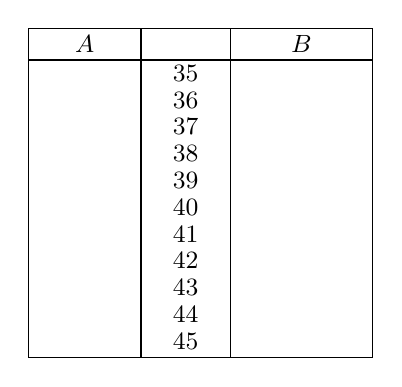
\begin{tikzpicture}[scale=0.95, semithick, every node/.style={inner sep=2.2pt, font=\small}]
  \draw (0,0) rectangle (4.6,-4.4);
  \draw (1.5,0) -- (1.5,-4.4);
  \draw (2.7,0) -- (2.7,-4.4);
  \draw (0,-0.42) -- (4.6,-0.42);
  \node at (0.75,-0.21) {$A$};
  \node at (3.65,-0.21) {$B$};
  \foreach \i/\s in {0/35,1/36,2/37,3/38,4/39,5/40,6/41,7/42,8/43,9/44,10/45} {
    \node at (2.1,{-0.42-(\i+0.5)*0.358}) {$\s$};
  }
\end{tikzpicture}
\end{center}
\nopagebreak[4]
\end{question}
\begin{question}
\gkti{18}已知椭圆 $\dfrac{x^2}{a^2}+\dfrac{y^2}{b^2}=1$（$a>b>0$）的离心率为 $\dfrac{\sqrt3}{3}$，以原点为圆心、椭圆短半轴长为半径的圆与直线 $y=x+2$ 相切．

（1）求 $a$ 与 $b$；

（2）设该椭圆的左、右焦点分别为 $F_1$ 和 $F_2$，直线 $l_1$ 过 $F_2$ 且与 $x$ 轴垂直，动直线 $l_2$ 与 $y$ 轴垂直，交 $l_1$ 于点 $P$．求线段 $PF_1$ 的垂直平分线与 $l_2$ 的交点 $M$ 的轨迹方程，并指明曲线类型．

\end{question}
\begin{question}
\gkti{19}已知数列 $\{a_n\}$ 的前 $n$ 项和 $S_n=2n^2+2n$，数列 $\{b_n\}$ 的前 $n$ 项和 $T_n=2-b_n$．

（1）求数列 $\{a_n\}$ 与 $\{b_n\}$ 的通项公式；

（2）设 $c_n=a_{2n}^2\cdot b_n$，证明：当且仅当 $n\geqslant3$ 时，$c_{n+1}<c_n$．

\Needspace{0.4\textheight}
\end{question}
\begin{question}
\gkti{20}如图，$ABCD$ 是边长为 $2$ 的正方形，直线 $l$ 与平面 $ABCD$ 平行，$E$ 和 $F$ 是 $l$ 上的两个不同点，且 $EA=ED$，$FB=FC$．$E'$ 和 $F'$ 是平面 $ABCD$ 内的两点，$EE'$ 和 $FF'$ 都与平面 $ABCD$ 垂直．
\nopagebreak[4]
\begin{center}% 2009 年安徽卷文科第 20 题：正方形 ABCD 与平行直线 l 构成的六面体 ABCDEF。
% 来源 PDF：普通高考/2009/2009安徽文.pdf，SHA256 83b982d22fd84a0158f909bce3d1f62e1fa228868e7915ded21e7a5ed9774897
% 原页：第 2 页（A3 三栏）第 2 栏中部，印刷页 498。
% 重绘依据：正方形按斜投影画成平行四边形，A 左下、B 右下、C 右上、D 左上；l 为 AB 上方的水平直线，
%   E、F 在 l 上（F 在右、超出正方形右边界）；E′、F′ 在正方形平面内的中线上，
%   EE′、FF′ 画虚线，DC 画虚线（被遮挡）；实线为 AB、BC、AD 与 E、F 到 A、D、B、C 的连线。
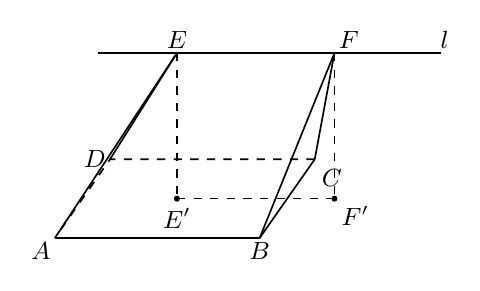
\begin{tikzpicture}[scale=1.0, semithick, every node/.style={inner sep=1.3pt, font=\small}]
  \coordinate (A) at (0,0);
  \coordinate (B) at (2.6,0);
  \coordinate (C) at (3.3,1.0);
  \coordinate (D) at (0.7,1.0);
  \coordinate (E) at (1.55,2.35);
  \coordinate (F) at (3.55,2.35);
  \coordinate (Ep) at (1.55,0.5);
  \coordinate (Fp) at (3.55,0.5);
  % 直线 l
  \draw (0.55,2.35) -- (4.9,2.35);
  \node[above] at (4.95,2.35) {$l$};
  % 正方形
  \draw (A) -- (B) -- (C);
  \draw[dashed] (C) -- (D) -- (A);
  % 棱
  \draw (A) -- (E);
  \draw (D) -- (E);
  \draw (B) -- (F);
  \draw (C) -- (F);
  \draw (E) -- (F);
  % 垂线
  \draw[dashed] (E) -- (Ep);
  \draw[dashed] (F) -- (Fp);
  % 中线
  \draw[dashed] (Ep) -- (Fp);
  \fill (Ep) circle (1.1pt);
  \fill (Fp) circle (1.1pt);
  \node[below left] at (A) {$A$};
  \node[below] at (B) {$B$};
  \node[anchor=north west] at ([xshift=1pt,yshift=-2pt]C) {$C$};
  \node[left] at (D) {$D$};
  \node[above] at (E) {$E$};
  \node[anchor=south west] at (F) {$F$};
  \node[below] at ([yshift=-2pt]Ep) {$E'$};
  \node[anchor=north west] at ([xshift=1pt,yshift=-1pt]Fp) {$F'$};
\end{tikzpicture}
\end{center}
\nopagebreak[4]
（1）证明：直线 $E'F'$ 垂直且平分线段 $AD$；

（2）若 $\angle EAD=\angle EAB=60^\circ$，$EF=2$，求多面体 $ABCDEF$ 的体积．

\end{question}
\begin{question}
\gkti{21}已知函数 $f(x)=x-\dfrac2x+1-a\ln x$，$a>0$．

（1）讨论 $f(x)$ 的单调性；

（2）设 $a=3$，求 $f(x)$ 在区间 $[1,\mathrm e^2]$ 上值域，其中 $\mathrm e=0.71828\cdots$ 是自然对数的底数．

\end{question}